\section{Vista Conceptual}\label{sec:vista-conceptual}

La Vista Conceptual brinda una descripción general de la plataforma y presenta los principales conceptos asociados.

\subsection{Descripción General de la Plataforma}

La solución \solucion cuenta con un componente central y un componente móvil, e interactúa con nodos periféricos y sistemas externos. Estos elementos brindan funcionalidades a ciudadanos pertenecientes a empresas transportistas, choferes, funcionarios, autoridades, administradores y público en general \cite{LINS2026}.

Las funcionalidades para las empresas transportistas se ofrecen mediante un frontoffice web del componente central. El responsable de una empresa puede gestionar su perfil, sus vehículos, permisos, inspecciones, guías de viaje e infracciones. La aplicación móvil permite que los choferes consulten el viaje asignado y registren el comienzo, la finalización, cargas o descargas parciales e incidentes, incluso cuando no disponen de conectividad.

Los funcionarios acceden a un frontoffice web para gestionar empresas, fiscalizar permisos y vehículos, monitorear viajes y resolver casos de fiscalización. Las autoridades utilizan un backoffice web para consultar reportes e indicadores. Los administradores utilizan el mismo backoffice para gestionar usuarios, roles, nodos periféricos y parámetros de las reglas de fiscalización.

Los nodos de balanzas suministran los pesajes registrados en los peajes y los nodos de tracking reportan periódicamente la posición de los vehículos. La Plataforma de Interoperabilidad permite consultar datos de organismos públicos, mientras que Usuario gub.uy proporciona la autenticación de ciudadanos y funcionarios.

\begin{figure}[ht]
    \centering
    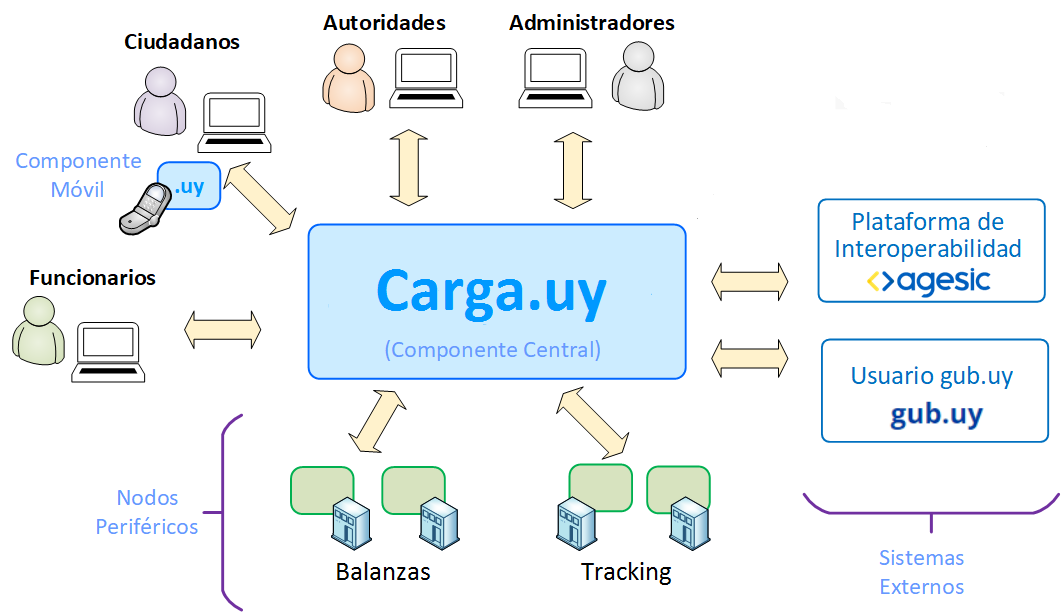
\includegraphics[width=15cm]{figures/descripcion-general.png}
    \caption{Descripción general de carga.uy}
    \label{fig:descr_general_plat}
\end{figure}

\subsection{Modelo Conceptual}

Los conceptos centrales son Usuario (Ciudadano, Funcionario, Administrador y Autoridad), Rol, Responsable, Chofer, Empresa, Vehículo, Permiso, ITV, Guía, Rubro, Tipo de Carga, Viaje, Evento (de viaje, incidente y de posición), Balanza, Peaje, Pesaje, Norma de Fiscalización, Caso de Fiscalización, Evidencia, Notificación, Descargo, Resolución, Pista de Auditoría e Informe. Un responsable representa a una empresa, que posee vehículos habilitados por un permiso e inspeccionados mediante la ITV. La empresa emite Guías que amparan viajes, asignados a un vehículo y conducidos por un chofer. Los eventos y pesajes asociados a los viajes constituyen evidencia para que las normas de fiscalización detecten posibles incumplimientos. Cada detección genera un caso que se notifica a la empresa, puede recibir un descargo y es resuelto por un funcionario, quedando sus acciones registradas en la pista de auditoría.

Los usuarios que se autentican con el mecanismo interno (autoridades y administradores) se agrupan bajo Usuario Backoffice, que es el único que guarda credenciales propias; funcionarios y ciudadanos se autentican con Usuario gub.uy.

\pendiente{en el monitoreo el tutor sugirió evaluar que la balanza tenga la ubicación y que Peaje y Balanza queden en relación 1 a 1, y dejar el modelo de dominio en pausa. Decidir si se aplica antes de la entrega.}

\begin{sidewaysfigure}
    \centering
    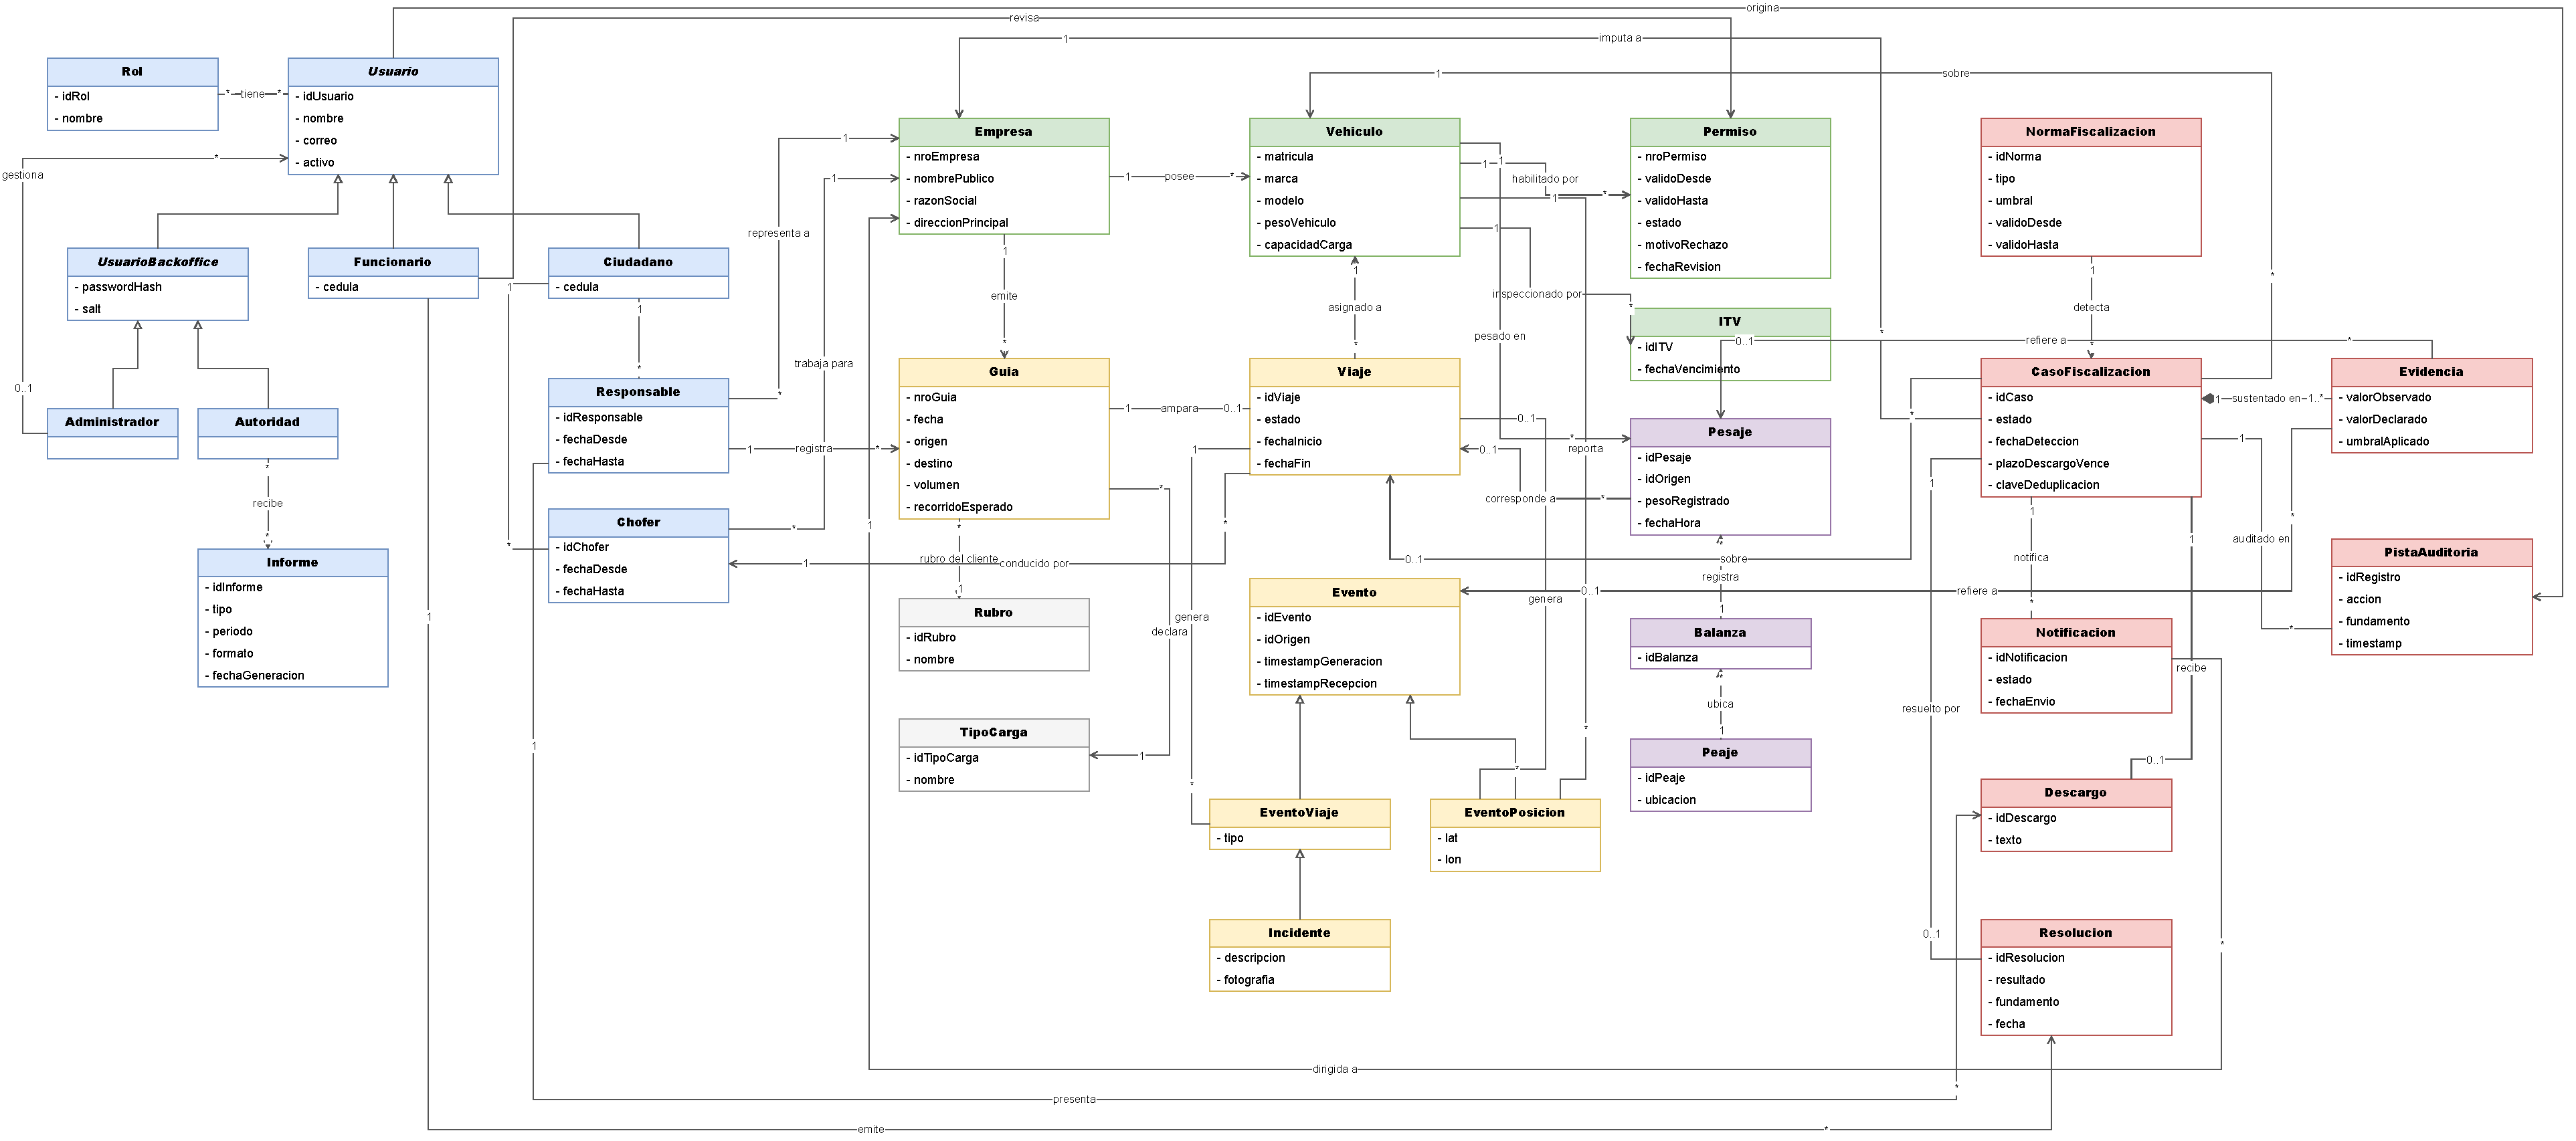
\includegraphics[width=0.98\textheight]{figures/modelo-conceptual.pdf}
    \caption{Modelo conceptual de carga.uy}
    \label{fig:modelo_conceptual}
\end{sidewaysfigure}
